\chapter{Spesies Kimia, Alami dan Sintetis}\label{ch:g10:chemical-species}

Sesendok es krim vanila. Rasanya mungkin berasal dari polong hitam
sejenis anggrek tropis, yang dipetik, diperam, dan direndam dalam alkohol
berbulan-bulan; atau mungkin berasal dari pabrik yang membuat perisa itu
dari bubur kayu atau dari minyak bumi. Cicipi keduanya berdampingan, dan
rasa utamanya sama --- dengan alasan yang kuat: \omterm{def:g7:atoms-and-molecules:molecule}{molekul} yang berasa
vanila, yaitu vanilin, adalah \omterm{def:g7:atoms-and-molecules:molecule}{molekul} yang persis sama, bagaimana pun
cara memperolehnya. Bab ini menunjukkan cara para ahli kimia mengambil
sebuah spesies dari tumbuhan, cara mereka membuatnya, dan cara mereka
memeriksa bahwa yang mereka miliki memang yang mereka kira.

\begin{recall}
\omterm{def:g6:pure-substances-and-mixtures:species}{Spesies kimia} adalah satu jenis zat tertentu; \omterm{def:g6:pure-substances-and-mixtures:pure-substance}{zat murni} mengandung satu
spesies dan memiliki tetapan yang tetap, seperti suhu leleh dan suhu
didihnya (\cref{ch:g6:pure-substances-and-mixtures}). Cairan \omterm{def:g6:solutions-and-solubility:miscible}{dapat
bercampur} atau \omterm{def:g6:solutions-and-solubility:miscible}{tidak dapat bercampur}, dan setiap \omterm{def:g6:solutions-and-solubility:solute}{zat terlarut} memiliki
\omterm{def:g6:solutions-and-solubility:solubility}{kelarutannya} sendiri dalam setiap \omterm{def:g6:solutions-and-solubility:solute}{pelarut}
(\cref{ch:g6:solutions-and-solubility}). \omterm{def:g7:identifying-substances:chromatography}{Kromatografi kertas} memisahkan
zat-zat warna sebuah \omterm{def:g6:pure-substances-and-mixtures:mixture}{campuran} (\cref{ch:g7:identifying-substances}).
\end{recall}

\begin{omfigure}
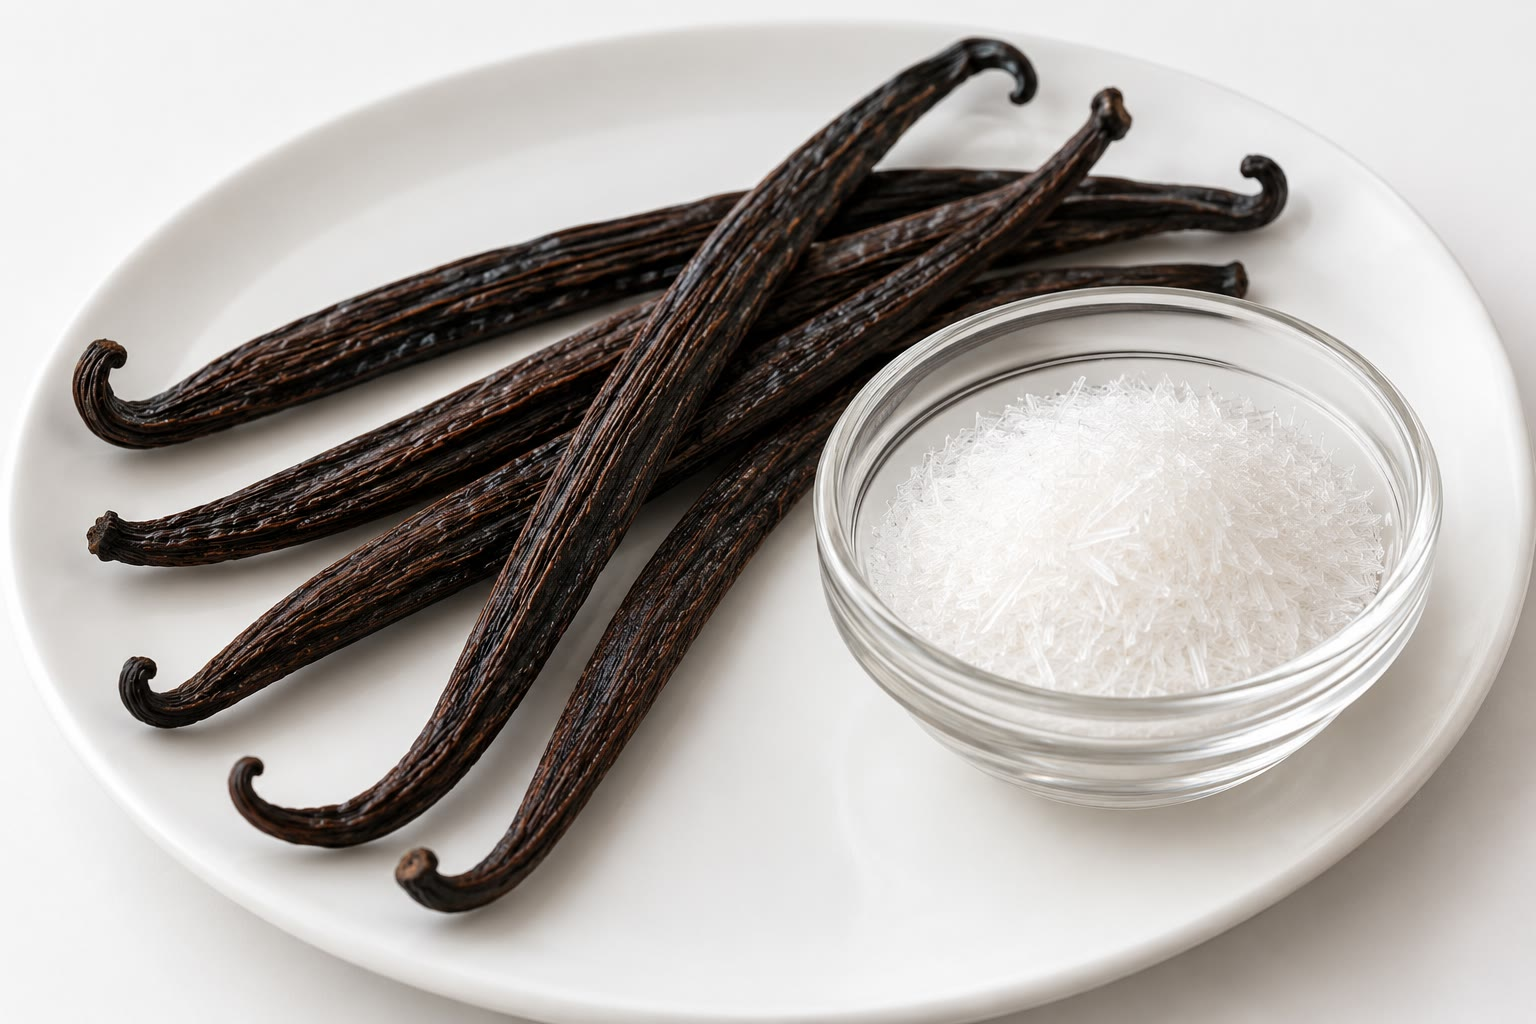
\includegraphics[width=0.55\linewidth]{images/book1/ai/g10-vanilla.jpg}

{\small Polong vanili dan kristal putih vanilin: \omterm{def:g7:atoms-and-molecules:molecule}{molekul} yang sama, dari
tumbuhan maupun dari pabrik.}
\end{omfigure}

\section{Spesies alami dan sintetis}

\begin{definition}[Spesies alami dan sintetis]\label{def:g10:chemical-species:natural}
Sebuah \emph{spesies alami}\index{spesies alami} adalah \omterm{def:g6:pure-substances-and-mixtures:species}{spesies kimia}
yang dibuat oleh makhluk hidup atau ditemukan apa adanya di alam. Sebuah
\emph{spesies sintetis}\index{spesies sintetis} dibuat oleh para ahli
kimia dari spesies-spesies lain melalui \omterm{def:g7:chemical-reactions:reaction}{reaksi kimia}. Spesies sintetis
dapat identik dengan spesies alami (vanilin sintetis), atau tidak
memiliki padanan di alam (sebagian besar obat dan \omterm{def:g8:plastics:plastic}{plastik}).
\end{definition}

\begin{proposition}[Spesies sama, sifat sama]\label{prop:g10:chemical-species:same}
Sebuah \omterm{def:g6:pure-substances-and-mixtures:species}{spesies kimia} memiliki sifat yang sama apa pun asalnya: vanilin
yang dibuat di pabrik dan vanilin yang diekstraksi dari polong memiliki
rumus yang sama, titik leleh yang sama, bau yang sama. Yang dapat
berbeda adalah apa yang menyertainya: ekstrak alami adalah \omterm{def:g6:pure-substances-and-mixtures:mixture}{campuran},
dengan banyak spesies lain yang mengubah rasanya.
\end{proposition}

\begin{history}[Dari kulit pohon dedalu sampai aspirin, 1828--1899]
Selama berabad-abad, kulit pohon dedalu dikunyah untuk melawan demam dan
nyeri. Pada tahun 1828 seorang ahli kimia mengekstraksi spesies aktifnya,
salisin; para ahli kimia kemudian mengubahnya menjadi asam salisilat,
yang manjur tetapi mengiritasi lambung. Pada tahun 1897, di sebuah
perusahaan zat warna dan obat, Felix Hoffmann membuat \omterm{def:g10:chemical-species:natural}{spesies sintetis}
yang lebih lembut dari asam salisilat: asam asetilsalisilat, yang dijual
sejak 1899 sebagai aspirin. Aspirin tidak memiliki sumber alami: aspirin
adalah spesies yang sepenuhnya sintetis.
\end{history}

\section{Mengekstraksi sebuah spesies}

\begin{definition}[Ekstraksi dan ekstraksi cair--cair]\label{def:g10:chemical-species:extraction}
Sebuah \emph{ekstraksi}\index{ekstraksi} mengambil sebuah \omterm{def:g6:pure-substances-and-mixtures:species}{spesies kimia}
dari bahan yang mengandungnya, biasanya dengan melarutkannya dalam
\omterm{def:g6:solutions-and-solubility:solute}{pelarut} yang dipilih dengan baik. Dalam
\emph{ekstraksi cair--cair}\index{ekstraksi cair--cair}, spesies yang
\omterm{def:g2:mixing-and-dissolving:dissolve}{larut} dalam satu cairan dipindahkan ke cairan kedua, yang \omterm{def:g6:solutions-and-solubility:miscible}{tidak dapat
bercampur} dengan cairan pertama, tempat spesies itu lebih mudah \omterm{def:g2:mixing-and-dissolving:dissolve}{larut};
kedua cairan lalu dipisahkan dengan corong pisah.
\end{definition}

\begin{example}[Ekstraksi sehari-hari]\label{ex:g10:chemical-species:everyday}
Menyeduh teh adalah \omterm{def:g10:chemical-species:extraction}{ekstraksi} dengan air panas (infusa); merendam polong
vanili dalam alkohol adalah \omterm{def:g10:chemical-species:extraction}{ekstraksi} dengan etanol (maserasi); merebus
sayuran untuk membuat kaldu adalah \omterm{def:g10:chemical-species:extraction}{ekstraksi} yang lain lagi (dekok).
\end{example}


\begin{definition}[Distilasi dan hidrodistilasi]\label{def:g10:chemical-species:distillation}
Sebuah \emph{distilasi}\index{distilasi} memanaskan \omterm{def:g6:pure-substances-and-mixtures:mixture}{campuran} cair sampai
mendidih, mengubah uapnya kembali menjadi cairan di dalam kondensor
yang didinginkan dengan air mengalir, dan menampung cairan itu, yaitu
distilat. Sebuah \emph{hidrodistilasi}\index{hidrodistilasi} mendidihkan
bahan tumbuhan dalam air: uap air membawa spesies-spesies harum dari
tumbuhan itu, yang memisah dari air di dalam distilat sebagai lapisan
berminyak, yaitu minyak atsiri.
\end{definition}

\begin{omfigure}
\begin{tikzpicture}[font=\small, scale=0.95]
  \pic[transform shape] at (0,0) {heatingmantle};
  \pic[transform shape] at (0,0) {rbflask={0.55}{omWater!70}};
  \foreach \x/\y in {-0.45/0.35,-0.1/0.55,0.3/0.3,0.5/0.7,-0.6/0.75,0.1/0.9,-0.25/0.2}
    \fill[green!45!black!70] (\x,\y) ellipse (0.09 and 0.04);
  \pic[transform shape] (s) at (0,3.0) {stillhead};
  \pic[transform shape] at ($(s-top)+(0,-0.75)$) {thermometer};
  \pic[transform shape, rotate=-20] (c) at (s-arm) {liebig={3.2}};
  \coordinate (cend) at ($(s-arm)+(-20:3.2)$);
  \pic[transform shape] (a) at (cend) {adapter};
  \pic[transform shape] at ($(a-tip)+(0,-2.3)$) {erlenmeyer={0.18}{omWater!70}};
  \fill[yellow!60!orange!60] ($(a-tip)+(-0.827,-2.3+0.47)$) -- ($(a-tip)+(0.827,-2.3+0.47)$) -- ($(a-tip)+(0.779,-2.3+0.6)$) -- ($(a-tip)+(-0.779,-2.3+0.6)$) -- cycle;
  \draw[<-, omProp, thick] (-0.55,0.55) -- (-2.2,0.9) node[left, text=black, align=right]
    {air dan\\ bunga lavender};
  \draw[<-, omProp, thick] (1.35,-0.6) -- (2.2,-1.1) node[right, text=black]
    {mantel pemanas};
  \draw[<-, omProp, thick] (0.1,4.2) -- (-1.2,4.6) node[left, text=black] {termometer};
  \draw[<-, omProp, thick] ($(s-arm)+(-20:1.6)+(0,0.32)$) -- ++(0.6,1.0) node[above, text=black]
    {kondensor berpendingin air mengalir};
  \draw[<-, omProp, thick] ($(a-tip)+(0.4,-1.88)$) -- ++(1.1,0.2) node[right, text=black, align=left]
    {distilat: minyak atsiri\\ terapung di atas air};
\end{tikzpicture}

{\small \omterm{def:g10:chemical-species:distillation}{Hidrodistilasi} lavender. Uap air membawa minyak atsiri ke dalam
kondensor; distilatnya memisah menjadi lapisan tipis minyak di atas
air.}
\end{omfigure}

\begin{method}[Memilih pelarut ekstraksi]\label{met:g10:chemical-species:solvent}
Untuk \omterm{def:g10:chemical-species:extraction}{ekstraksi cair--cair} sebuah spesies dari air, \omterm{def:g6:solutions-and-solubility:solute}{pelarutnya} harus:
\begin{enumerate}
  \item melarutkan spesies itu jauh lebih baik daripada air;
  \item \omterm{def:g6:solutions-and-solubility:miscible}{tidak dapat bercampur} dengan air, sehingga terbentuk dua lapisan;
  \item sesedikit mungkin berbahaya, dan mudah dihilangkan sesudahnya
        (titik didih yang rendah memungkinkannya \omterm{def:g3:separating-mixtures:evaporate}{menguap}).
\end{enumerate}
Lapisan mana yang berada di atas ditentukan oleh massa jenisnya: cairan
yang massa jenisnya lebih kecil terapung.
\end{method}

\begin{example}[Pelarut untuk minyak lavender]\label{ex:g10:chemical-species:table}
% ledger: rho:cyclohexane, bp:cyclohexane, rho:ethyl-acetate, bp:ethyl-acetate, rho:CH2Cl2, bp:CH2Cl2, rho:ethanol, bp:ethanol, sol:linalool
Linalool, spesies utama minyak lavender, hanya \omterm{def:g2:mixing-and-dissolving:dissolve}{larut} sebanyak
\qty{1.6}{g/L} dalam air, tetapi sangat mudah \omterm{def:g2:mixing-and-dissolving:dissolve}{larut} dalam \omterm{def:g6:solutions-and-solubility:solute}{pelarut-pelarut}
di bawah ini:
\begin{center}
\small
\begin{tabular}{lccll}
\hline
\omterm{def:g6:solutions-and-solubility:solute}{pelarut} & massa \qty{1}{mL} & mendidih pada & dengan air & bahaya utama \\
\hline
sikloheksana & \qty{0.78}{g} & \qty{81}{\celsius} & tidak bercampur & mudah menyala, berbahaya \\
etil etanoat & \qty{0.90}{g} & \qty{77}{\celsius} & tidak bercampur & mudah menyala, iritan \\
diklorometana & \qty{1.33}{g} & \qty{40}{\celsius} & tidak bercampur & diduga karsinogen \\
etanol & \qty{0.79}{g} & \qty{78}{\celsius} & bercampur & mudah menyala \\
\hline
\end{tabular}
\end{center}
Etanol tidak dapat dipakai: etanol bercampur dengan air dan tidak
terbentuk lapisan. Dengan sikloheksana atau etil etanoat, lapisan
\omterm{def:g6:solutions-and-solubility:solute}{pelarutnya} berada di atas; dengan diklorometana, di bawah.
\end{example}

\begin{omfigure}
\begin{tikzpicture}[font=\small, scale=1.2]
  \pic[transform shape] at (0,0) {sepfunnel={omWater!70}{yellow!35!orange!35}};
  \draw[<-, omProp, thick] (0.55,2.1) -- (1.6,2.4) node[right, text=black, align=left]
    {sikloheksana dan minyaknya\\ (massa jenis lebih kecil, di atas)};
  \draw[<-, omProp, thick] (0.55,1.3) -- (1.6,1.2) node[right, text=black, align=left]
    {air, dikeluarkan\\ melalui keran};
  \draw[<-, omProp, thick] (0.25,0.52) -- (1.6,0.4) node[right, text=black] {keran};
\end{tikzpicture}

{\small Corong pisah setelah dikocok dan didiamkan: minyaknya telah
berpindah ke sikloheksana, di atas.}
\end{omfigure}

\begin{safety}{\ghs[0.8cm]{GHS02}\ghs[0.8cm]{GHS07}\ghs[0.8cm]{GHS08}\ghs[0.8cm]{GHS09}}
% ledger: ghs:cyclohexane
Sikloheksana: sangat mudah menyala (GHS02); dapat berakibat fatal jika
tertelan dan masuk ke saluran pernapasan, menyebabkan iritasi kulit dan
kantuk (GHS07, GHS08); sangat beracun bagi kehidupan akuatik (GHS09).
Dipakai di dalam lemari asam, jauh dari nyala api.
\end{safety}

\section{Kromatografi lapis tipis}

\begin{definition}[Kromatografi lapis tipis]\label{def:g10:chemical-species:tlc}
Yang disebut \emph{kromatografi lapis tipis}\index{kromatografi lapis tipis}
(KLT) memisahkan spesies-spesies sebuah \omterm{def:g6:pure-substances-and-mixtures:mixture}{campuran} pada pelat yang
dilapisi selapis tipis serbuk putih yang halus, yaitu
\emph{fase diam}\index{fase diam}. Totolan-totolan kecil sampel
diletakkan pada garis pensil di dekat bagian bawah; pelat itu berdiri di
dalam bejana tertutup berisi sedikit \omterm{def:g6:solutions-and-solubility:solute}{pelarut}, yaitu
\emph{eluen}\index{eluen}, yang naik melalui pelat dan membawa setiap
spesies sampai ketinggian yang bergantung pada spesiesnya. Bercak yang
tak berwarna kemudian ditampakkan, di bawah sinar ultraviolet atau
dengan uap iodin.
\end{definition}

\begin{definition}[Faktor retensi]\label{def:g10:chemical-species:retention-factor}
Yang disebut \emph{faktor retensi}\index{faktor retensi} sebuah bercak adalah
\[
  R_f = \frac{\text{jarak dari garis awal ke bercak}}
             {\text{jarak dari garis awal ke garis depan pelarut}},
\]
sebuah bilangan antara 0 dan 1. Untuk pelat, \omterm{def:g10:chemical-species:tlc}{eluen}, dan suhu tertentu,
setiap spesies memiliki $R_f$-nya sendiri.
\end{definition}

\begin{method}[Melakukan dan membaca KLT]\label{met:g10:chemical-species:tlc}
\begin{enumerate}
  \item Gambarlah garis awal dengan pensil, \qty{1}{cm} dari bagian
        bawah; letakkan setotol kecil setiap sampel dan setiap spesies
        pembanding di atasnya.
  \item Berdirikan pelat di dalam bejana, \omterm{def:g10:chemical-species:tlc}{eluen} di bawah garis; tutup
        bejananya.
  \item Angkat pelat ketika garis depan sekitar \qty{1}{cm} dari bagian
        atas; tandai garis depan itu segera; keringkan dan tampakkan.
  \item Ukur jarak-jaraknya dan hitung $R_f$ setiap bercak. Sampel yang
        memberikan satu bercak kemungkinan spesies murni; bercak yang
        setinggi bercak pembanding pada pelat yang sama kemungkinan besar
        adalah spesies itu.
\end{enumerate}
\end{method}

\begin{omfigure}
\begin{tikzpicture}[font=\small, scale=1.25]
  % the tank
  \pic[transform shape] at (0,0) {beaker={0.15}{omWater!80}};
  \fill[white] (-0.55,0.08) rectangle (0.55,1.92);
  \fill[omWater!80] (-0.55,0.08) rectangle (0.55,0.3);
  \draw[omGlass, line width=0.6pt] (-0.55,0.08) rectangle (0.55,1.92);
  \draw[black!60] (-0.55,0.42) -- (0.55,0.42);
  \foreach \x in {-0.3,0,0.3} \fill[black!70] (\x,0.42) circle (0.04);
  \fill[black!25] (-1.0,2.08) rectangle (1.0,2.18);
  \node[anchor=north, align=center] at (0,-0.15) {bejana, ditutup\\ dengan tutupnya};
  % the developed plate
  \begin{scope}[xshift=4.2cm]
    \pic[transform shape] at (0,0) {tlcplate};
    \draw[black!50, dashed] (-0.7,2.8) -- (0.7,2.8);
    \fill[omDef!70] (-0.35,1.36) ellipse (0.1 and 0.07);
    \fill[omDef!70] (-0.35,2.2) ellipse (0.1 and 0.07);
    \fill[omDef!70] (0,1.36) ellipse (0.1 and 0.07);
    \fill[omDef!70] (0.35,2.2) ellipse (0.1 and 0.07);
    \foreach \x/\l in {-0.35/O,0/L,0.35/A} \node[font=\footnotesize, anchor=north] at (\x,0.38) {\l};
    \draw[<->, omProp] (0.95,0.4) -- (0.95,1.36) node[midway, right, text=black, font=\footnotesize] {$d$};
    \draw[<->, omProp] (1.55,0.4) -- (1.55,2.8) node[midway, right, text=black, font=\footnotesize] {$D$};
    \draw[black!40, densely dotted] (-0.25,1.36) -- (0.95,1.36);
    \node[anchor=north, align=center] at (0.2,-0.15) {pelat yang sudah dikembangkan:\\ $R_f = d/D$};
  \end{scope}
\end{tikzpicture}

{\small KLT minyak lavender (O) di samping linalool (L) dan linalil
etanoat (A). Minyak itu memberikan dua bercak, setinggi kedua
pembanding: minyak itu mengandung kedua spesies. Untuk linalool,
$R_f = d/D$.}
\end{omfigure}

\section{Mengenali spesies dari tetapan fisikanya}

\begin{proposition}[Titik leleh memeriksa identitas dan kemurnian]\label{prop:g10:chemical-species:mp}
% ledger: mp:vanillin, mp:aspirin, mp:salicylic
Padatan murni meleleh dengan tajam pada suhunya sendiri: vanilin pada
sekitar \qty{82}{\celsius}, aspirin pada \qty{135}{\celsius}, asam
salisilat pada \qty{158}{\celsius}. Sampel yang tidak murni meleleh pada
suhu yang lebih rendah, dan dalam rentang beberapa derajat. Karena itu
mengukur titik leleh, di atas bangku \omterm{def:g9:periodic-table-first-look:metal}{logam} yang dipanaskan atau dengan
alat titik leleh, sekaligus mengenali sebuah padatan dan menunjukkan
apakah padatan itu murni.
\end{proposition}

\begin{inthelab}[Sebuah pelat KLT]
Para siswa menotolkan minyak lavender, linalool, dan linalil etanoat
pada sebuah pelat, mengembangkannya di dalam stoples tertutup dengan
\omterm{def:g6:pure-substances-and-mixtures:mixture}{campuran} \omterm{def:g6:solutions-and-solubility:solute}{pelarut} yang dipilih oleh guru, lalu menampakkannya di bawah
lampu ultraviolet, sambil memakai kacamata yang menahan sinar
ultraviolet. \omterm{def:g10:chemical-species:tlc}{Eluen} dipakai dan ditangani di dalam lemari asam.
\end{inthelab}

\begin{omfigure}
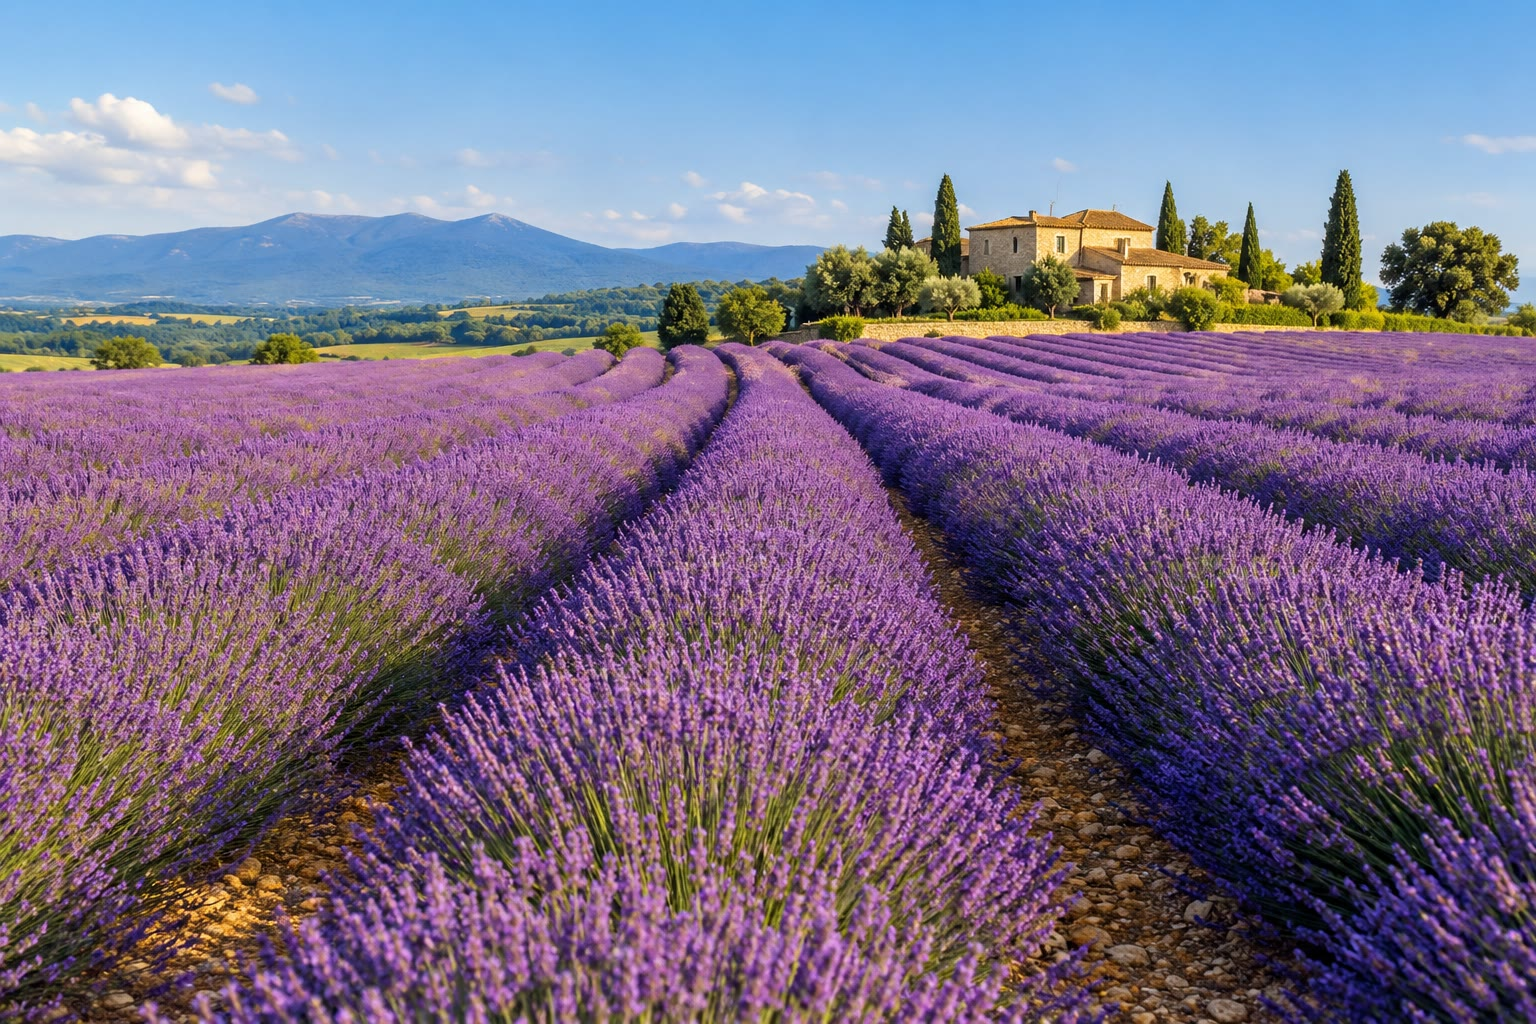
\includegraphics[width=0.55\linewidth]{images/book1/ai/g10-lavender-field.jpg}

{\small Ladang lavender yang sedang berbunga: \omterm{def:g5:raw-materials-and-recycling:raw-material}{bahan baku} minyak atsiri
lavender.}
\end{omfigure}

\section{Latihan}

\begin{exercise}[$\star$]\label{exo:g10:chemical-species:1}
\omterm{def:g10:chemical-species:natural}{Spesies alami} atau sintetis? Vanilin dari polong vanili; aspirin;
kafein dari biji kopi; vanilin yang dibuat di pabrik.
\end{exercise}

\begin{exercise}[$\star$]\label{exo:g10:chemical-species:2}
Mengapa vanilin sintetis dan vanilin alami memiliki titik leleh yang
sama?
\end{exercise}

\begin{exercise}[$\star$]\label{exo:g10:chemical-species:3}
Pada sebuah pelat KLT, garis depan \omterm{def:g6:solutions-and-solubility:solute}{pelarut} berada \qty{6.0}{cm} di atas
garis awal dan sebuah bercak \qty{2.4}{cm} di atasnya. Hitung $R_f$-nya.
\end{exercise}

\begin{exercise}[$\star$]\label{exo:g10:chemical-species:4}
Sebutkan peran kondensor dalam \omterm{def:g10:chemical-species:distillation}{distilasi}, dan jelaskan mengapa air
dingin masuk dari ujung bawahnya.
\end{exercise}

\begin{exercise}[$\star$]\label{exo:g10:chemical-species:5}
Sebutkan tiga syarat yang harus dipenuhi sebuah \omterm{def:g6:solutions-and-solubility:solute}{pelarut} \omterm{def:g10:chemical-species:extraction}{ekstraksi}.
\end{exercise}

\begin{exercise}[$\star\star$]\label{exo:g10:chemical-species:6}
Dengan tabel \omterm{def:g6:solutions-and-solubility:solute}{pelarut}, jelaskan mengapa etanol tidak dapat dipakai untuk
mengekstraksi linalool dari distilat, sedangkan sikloheksana dapat.
\end{exercise}

\begin{exercise}[$\star\star$]\label{exo:g10:chemical-species:7}
Dalam corong pisah, diklorometana dikocok dengan air. Lapisan mana yang
berada di atas? Berikan alasan dengan tabel itu.
\end{exercise}

\begin{exercise}[$\star\star$]\label{exo:g10:chemical-species:8}
Serbuk putih yang dijual sebagai aspirin mulai meleleh pada
\qty{126}{\celsius} dan meleleh seluruhnya pada \qty{132}{\celsius}.
Apa yang dapat kamu simpulkan?
\end{exercise}

\begin{exercise}[$\star\star$]\label{exo:g10:chemical-species:9}
Lihatlah gambar KLT dalam bab ini. Apa yang dikandung minyak lavender
itu? Spesies mana yang naik lebih tinggi?
\end{exercise}

\begin{exercise}[$\star\star$]\label{exo:g10:chemical-species:10}
Urutkan langkah-langkah memperoleh minyak lavender di laboratorium:
memisahkan lapisan-lapisan; \omterm{def:g10:chemical-species:distillation}{hidrodistilasi}; menambahkan sikloheksana ke
distilat dan mengocoknya; \omterm{def:g3:separating-mixtures:evaporate}{menguapkan} sikloheksana.
\end{exercise}

\begin{exercise}[$\star\star$]\label{exo:g10:chemical-species:11}
Mengapa garis awal pelat KLT digambar dengan pensil dan ditempatkan di
atas \omterm{def:g10:chemical-species:tlc}{eluen}?
\end{exercise}

\begin{exercise}[$\star\star\star$]\label{exo:g10:chemical-species:12}
Setelah \omterm{def:g10:chemical-species:extraction}{ekstraksi}, sikloheksana dihilangkan dengan pemanasan pelan,
sehingga tinggal minyaknya. Dengan titik didih sikloheksana dan titik
didih linalool (\qty{198}{\celsius}), jelaskan mengapa cara ini berhasil.
\end{exercise}

\begin{exercise}[$\star\star\star$]\label{exo:g10:chemical-species:13}
Sampel sintetis sebuah perisa memberikan satu bercak pada pelat KLT,
setinggi \omterm{def:g10:chemical-species:natural}{spesies alaminya}, dan meleleh dengan tajam pada suhu yang
tepat. Dua kesimpulan apa yang dapat kamu tarik?
\end{exercise}

\begin{exercise}[$\star\star\star$]\label{exo:g10:chemical-species:14}
Pada KLT yang sama, bercak A memiliki $R_f = 0.40$ dan garis depan
berada \qty{5.5}{cm} di atas garis awal. Pada ketinggian berapa bercak A?
Spesies lain memiliki $R_f = 0.75$: berapa jauh di atas bercak A
letaknya?
\end{exercise}

\begin{exercise}[$\star\star\star$]\label{exo:g10:chemical-species:15}
Sebanyak \qty{1.6}{g} linalool dapat \omterm{def:g2:mixing-and-dissolving:dissolve}{larut} dalam \qty{1}{L} air. Sebuah
distilat berisi \qty{200}{mL} air mengandung \qty{0.20}{g} linalool
terlarut. Apakah distilat itu jenuh? Berapa banyak lagi yang masih dapat
dilarutkannya? Mengapa air ini layak diekstraksi dengan sikloheksana
alih-alih dibuang?
\end{exercise}

\clearpage % keeps the heading with its problem box (it was stranded at a page foot)
\section{Soal: Harum Lavender}

\begin{problem}[{Soal akhir pekan --- dari sekeranjang bunga lavender
sampai beberapa tetes minyak atsiri, diperiksa dengan kromatografi}]
\label{pb:g10:chemical-species:1}
% ledger: rho:cyclohexane, bp:cyclohexane, rho:CH2Cl2, bp:linalool, ghs:cyclohexane
Di laboratorium sekolah, \qty{100}{g} bunga lavender segar
dihidrodistilasi dengan air. Distilatnya, yang keruh, dikocok dengan
\qty{20}{mL} sikloheksana di dalam corong pisah; lapisan sikloheksana
disimpan, dikeringkan, dan sikloheksananya \omterm{def:g3:separating-mixtures:evaporate}{diuapkan} dengan pemanasan
pelan. Yang tersisa adalah minyak atsiri lavender. Pakailah tabel
\omterm{def:g6:solutions-and-solubility:solute}{pelarut} dalam bab ini.

\medskip
\noindent\textbf{Bagian I --- \omterm{def:g10:chemical-species:distillation}{Hidrodistilasi}.}
\begin{enumerate}
  \item Apa peran air yang mendidih dalam \omterm{def:g10:chemical-species:distillation}{hidrodistilasi}?
  \item Apa peran kondensor? Dari mana air dingin masuk ke dalamnya?
  \item Distilat memperlihatkan lapisan tipis berminyak yang terapung di
        atas air. Apakah minyak itu \omterm{def:g6:solutions-and-solubility:miscible}{dapat bercampur} dengan air? Apakah
        massa jenisnya lebih besar atau lebih kecil daripada air?
  \item Mengapa distilat itu tidak dituang begitu saja untuk mendapatkan
        minyaknya?
\end{enumerate}

\medskip
\noindent\textbf{Bagian II --- \omterm{def:g10:chemical-species:extraction}{Ekstraksi}.}
\begin{enumerate}[resume]
  \item Mengapa sikloheksana \omterm{def:g6:solutions-and-solubility:solute}{pelarut} yang cocok untuk \omterm{def:g10:chemical-species:extraction}{ekstraksi} ini?
  \item Dapatkah etanol dipakai sebagai gantinya? Jelaskan.
  \item Setelah dikocok dan didiamkan, apakah lapisan sikloheksana berada
        di atas atau di bawah? Bagaimana jika memakai diklorometana?
  \item Berikan dua tindakan pencegahan yang dituntut oleh piktogram
        sikloheksana.
  \item Mengapa sikloheksana dapat \omterm{def:g3:separating-mixtures:evaporate}{diuapkan} tanpa kehilangan linalool,
        yang mendidih pada \qty{198}{\celsius}?
\end{enumerate}

\medskip
\noindent\textbf{Bagian III --- Kromatografi.}
Minyak itu, linalool murni (L), dan linalil etanoat murni (A) ditotolkan
pada sebuah pelat KLT. Setelah dikembangkan, garis depan berada
\qty{6.0}{cm} di atas garis awal. Minyak itu memberikan dua bercak, pada
\qty{2.4}{cm} dan \qty{4.5}{cm}; bercak L berada pada \qty{2.4}{cm},
bercak A pada \qty{4.5}{cm}.
\begin{enumerate}[resume]
  \item Hitung $R_f$ linalool dan linalil etanoat.
  \item Apa yang dikandung minyak itu, sejauh yang ditunjukkan pelat ini?
  \item Apakah minyak lavender \omterm{def:g6:pure-substances-and-mixtures:pure-substance}{zat murni}?
  \item Mengapa pembanding-pembanding itu ditotolkan pada pelat yang sama
        dengan minyaknya?
  \item Linalool sintetis ditotolkan pada pelat lain yang dikembangkan
        dalam kondisi yang sama: bercaknya memiliki $R_f = 0.40$. Apa yang
        dapat disimpulkan?
\end{enumerate}

\medskip
\noindent\textbf{Bagian IV --- Berapa banyak minyaknya?}
Minyak yang diperoleh mengisi \qty{1.0}{mL}; \qty{1}{mL} minyak ini
beratnya \qty{0.90}{g}.
\begin{enumerate}[resume]
  \item Berapa massa minyak yang diperoleh?
  \item Berapa persen massa bunga itu?
  \item Berapa massa bunga yang diperlukan untuk \qty{100}{g} minyak?
  \item Minyak itu disebut ``alami''. Dalam arti apa hal ini benar?
        Apakah linaloolnya berbeda dari linalool sintetis?
  \item Nyatakan massa minyak atsiri yang diperoleh dari \qty{100}{g}
        bunga.
\end{enumerate}
\end{problem}
